%%%%%%%%%%%%%%%%%%%%%%%%%%%%%%%%%%%%%%%%%%%%%%%%%%%%%%%%%%%%%%
%% LaTeX template for the science justification to be       %%
%%     submitted as part of a regular ALMA proposal.        %%
%% This template should also be used for a ToO, DDT, VLBI,  %%
%%     or Phased Array ALMA proposal, but NOT for Large     %%
%%     Programs (these have a separate template)            %%
%%                                                          %%
%%                      ALMA Cycle 10                       %%
%%                                                          %%
%%%%%%%%%%%%%%%%%%%%%%%%%%%%%%%%%%%%%%%%%%%%%%%%%%%%%%%%%%%%%%

%%%%%%%%%%%%%%%%%%%%%%%%%%%%%%%%%%%%%%%%%%%%%%%%%%
%%%%% How to convert this document to PDF %%%%%%%%
%%%%%%%%%%%%%%%%%%%%%%%%%%%%%%%%%%%%%%%%%%%%%%%%%%

% If your figures are stored as PostScript files, you can use the 
% following commands to generate a PDF file of your proposal:

%% latex file.tex
%% dvips file.dvi
%% ps2pdf file.ps file.pdf 


% If your figures are PDF images or bitmap pictures in PNG, JPG, or GIF format,
% you can use the pdflatex command to generate a PDF file from this template
% (note, however, that the pdflatex command does not handle PostScript files):

% pdflatex file.tex

% Warnings: 
%           1. You must make sure that PDF output generated from this
%              template is complete both when displayed with a viewer 
%              (acroread, for example) and when printed on paper.
%              LaTeX installations vary greatly and therefore it might 
%              not be possible to get all proposals to come out 
%              correctly with a single text page layout. 
%              In some cases you will have to adjust the 
%              \topmargin=-7mm command in the template to center the 
%              text vertically in the page.  
%           2. The scientific justification, figures, tables, references,
%              and public outreach statement must all fit within the
%              4-page limit.
%           3. You are free to include colour images in your proposal justification.
%              Proposals are distributed to ALMA Review Panels and to distributed
%              peer review reviewers in electronic form.
%              However, the scientific content of the images should still remain
%              clear when displayed or printed in black and white.
%           4. This template is for Regular, ToO, DDT, mm-VLBI, or Phased Array
%              ALMA proposals, but NOT for Large Programs: these have a
%              separate template with more sections, and is available from the
%              ALMA Science Portal: http://almascience.org


%%%%%%%%%%%%%%%%%%%%%%%%%%%%%%%%%%%%%%%%%%%%%%
%%%%% Default format: 12pt single column %%%%%
%% 12pt is the minimum font size allowed !! %%
%% This applies to everything, including    %%
%% references, figure captions, and tables  %%
%% ==> Proposals not compliant to this will %%
%%     be rejected. See Section 5.3.1 in    %%
%%     the ALMA Proposer's Guide            %%
%%%%%%%%%%%%%%%%%%%%%%%%%%%%%%%%%%%%%%%%%%%%%%

\documentclass[12pt,a4paper]{article}  %% DO NOT CHANGE to 11pt or less !

\usepackage{natbib}
\usepackage{hyperref}
\usepackage{graphics,graphicx}
\usepackage{xspace}
\usepackage{amsmath,amssymb}
\newcommand{\msun}{\ensuremath{\mathrm{M}_\odot}\xspace}
\newcommand{\kms}{\ensuremath{\mathrm{km~s}^{-1}}\xspace}
\newcommand{\percc}{\ensuremath{\mathrm{cm}^{-3}}\xspace}
\newcommand{\persc}{\ensuremath{\mathrm{cm}^{-2}}\xspace}

\usepackage[table]{xcolor}% http://ctan.org/pkg/xcolor



%%%%%%%%%%%%%%%%%%%%%%%%%%%%
%%%%%% Page dimensions %%%%%
%%%%%%  DO NOT CHANGE  %%%%%
%%%%%%%%%%%%%%%%%%%%%%%%%%%%

\textheight=247mm
\textwidth=180mm
\topmargin=-7mm
\oddsidemargin=-10mm
\evensidemargin=-10mm
\parindent 10pt

%%%%%%%%%%%%%%%%%%%%%%%%%%%%%
%%%%% Start of document %%%%% 
%%%%%%%%%%%%%%%%%%%%%%%%%%%%%

\begin{document}
\pagestyle{plain}
\pagenumbering{arabic}
\newcommand{\arcsec}{"}
 
% The title, abstract and list of investigators should NOT be included in the
% Scientific justification. The title and abstract are put automatically on the cover page.

%%%%%%%%%%%%%%%%%%%%%%%%%%%%%%%%%%%%%%%%%
%%%%% Body of science justification %%%%%
%%%%%%%%%%%%%%%%%%%%%%%%%%%%%%%%%%%%%%%%%

%% ENTER TEXT, FIGURES AND TABLES BELOW
%% Minimum font size for all text, references, figure captions, and tables is 12pt
%% Proposals not compliant to this will be rejected. See Section 5.3.1 in the ALMA Proposer's Guide.

\section{Scientific justification}

\textcolor{red}{The DDT proposal is a work in progress and will not be submitted until after the formal ALMA deadline}

% ALMA uses two systems to review the proposals submitted in the Main Call.
% All proposals requesting less than 50 h on the 12-m Array and all ACA stand-alone proposals
% requesting less than 150 h on the 7-m Array will be reviewed by Distributed peer review
% (see Sections 5.7.1 and 1.2.2 of the Proposer's Guide).
% All Large Programs will be reviewed by Panels. 
% Additionally, both systems will follow a dual-anonymous procedure, in which the proposers
% do not know who are the reviewers and the reviews do not who are the proposers.
%
% Please refer to the guidelines before writing your proposal:
%     https://almascience.org/proposing/alma-proposal-review/dual-anonymous
%
% In the following part, describe the scientific background of the project,
% pertinent references and previous work relevant to this 
% proposal, together with any figures and tables that you judge necessary
% (use the following two examples as templates, or remove)
% Please do not disclose the name(s) of the proposer(s), and write the proposal in a way
% such that the proposer(s) cannot be identified. 
 
%-----------------------------Figure Start---------------------------

% The 'scale' parameter below allows you to scale the figure so that it fits within the page.
% In this case the figure was scaled to 20% of its original size.
% Note: for .png files one has to use pdflatex, not classic latex
%
% Minimum font size for references: 12pt 
% Proposals not compliant to this will be rejected. See Section 5.3.1 in the ALMA Proposer's Guide.
We detected a compact (barely resolved at 1\arcsec~ resolution) millimeter source with extremely broad line width in the Galactic Center.
This source, G0.02467-0.0727, is detected both in continuum and in very broad line emission (FWHM $\sim165~\kms$) in emission lines of CS and SO.
It is not detected at any other wavelength from X-ray to radio.
In a submitted paper \citep{Ginsburg2024}, we have evaluated many hypotheses for the nature of this source, and find that none are presently satisfactory.
We request DDT observations to classify the source, or at least narrow down the possibilities.
In just under 15h, we will resolve the source with 10$\times$ better resolution and we will definitively measure the gas excitation.
These measurements will provide definitive tests of several hypotheses and will drive further hypothesis formation for this as-yet unclassified source.

\textbf{Why DDT, why now?}
As you will read below, this object is truly unique, defying classification.
Despite the many telescopes and surveys that have observed the Galactic center, only ALMA has detected it, and it did so in many lines and continuum in a very brief integration.
It is essential to follow up this object in the next moderately long-baseline campaign (C6 this southern winter) to narrow down the space of available models and determine what other wavelength observations are possible.
Furthermore, it is essential to constrain the source size to determine if the object is a viable target for the Event Horizon Telescope.

\textbf{Source property summary:}
The continuum emission has a spectral index $\alpha\approx3.3$, suggesting that it is from dust.
It is detected in all three ALMA observations that overlap on the sky (two 12M data sets in B3, one 7M in B7).
The line emission is detected in several transitions of CS and SO and exhibits a line width FWHM $\approx165$ \kms.  The line profile appears Gaussian.
The emission is weakly spatially resolved, coming from an area on the sky $\lesssim1"$ in diameter ($\lesssim10^4$ AU at the distance of the GC).
The centroid velocity $v_{LSR}\approx40-50$ \kms, which suggests the object is genuinely in the Galactic Center and is possibly associated with the 50 \kms cloud.
There is a tentative detection (10$\sigma$ accounting for statistical error only; the systematic errors are difficult to quantify) of a velocity gradient of 1100 \kms pc$^{-1}$.
With multiple SO lines detected, and assuming LTE conditions, we estimate a gas temperature of 13 K, much colder than seen in typical Galactic Center clouds.
However, with the limited set of lines presently detected, it is also possible that the emission is coming from low-density, subthermally excited gas.
Despite the high velocity dispersion, no emission is observed from SiO, suggesting that there are no strong ($\gtrsim10~\kms$) shocks in the molecular gas.
There are no detections at other wavelengths, including X-ray with Chandra, XMM-Newton, and NUSTAR, infrared with HST and Spitzer, and radio with VLA and MEERKAT.

We consider several explanations for this source, including protostellar outflow, explosive outflow, collapsing cloud, evolved star, stellar collision, high-velocity cloud, intermediate mass black hole, and background galaxy.
Most of these conceptual models are inconsistent with the data in at least one way, but the data are not presently very constraining.
In this proposal, we will observe additional lines of the detected species (CS and SO) to measure the source excitation and additional continuum bands to verify the dusty nature of the source.
We will observe at higher resolution to determine whether the possible velocity gradient is real and to resolve the structure, whether it's an outflow, a disk, or something else entirely.

The most exciting possibilities for this source are that it is an intermediate mass black hole (IMBH) or it is a very massive, very obscured isolated young stellar object.
In either of such cases, we expect to see a velocity gradient at higher resolution - for an IMBH, from the disk, and for a YSO, from the outflow.
Observations at higher physical resolution ($\sim1600$ AU proposed) will be able to definitively rule out the IMBH model.
The archival data have 2" (16,000 AU) resolution, and we were able to measure a 2000 AU offset between the red- and blue-shifted lobes of the object by centroiding, so we expect to be able to measure down to at least $\sim200$ AU with the proposed higher-resolution and higher-sensitivity data.
An orbit of $v=165$ \kms at $r=200$ AU requires a central object with $M\sim6000$ \msun, so we should resolve the disk kinematically for any more massive object.

\begin{figure}
    \centering
    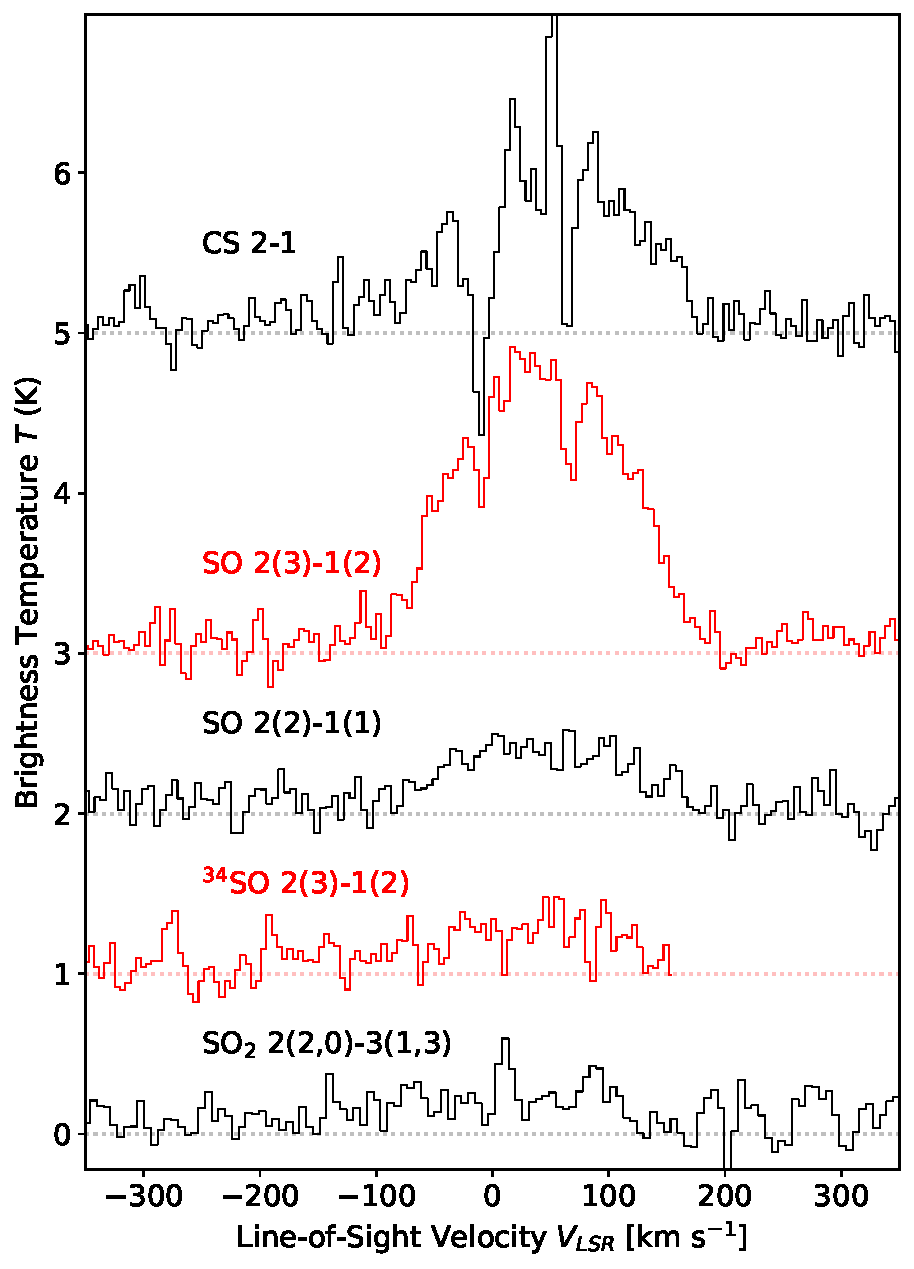
\includegraphics[width=0.49\textwidth]{figures/CSandSO_Overlays.pdf}
    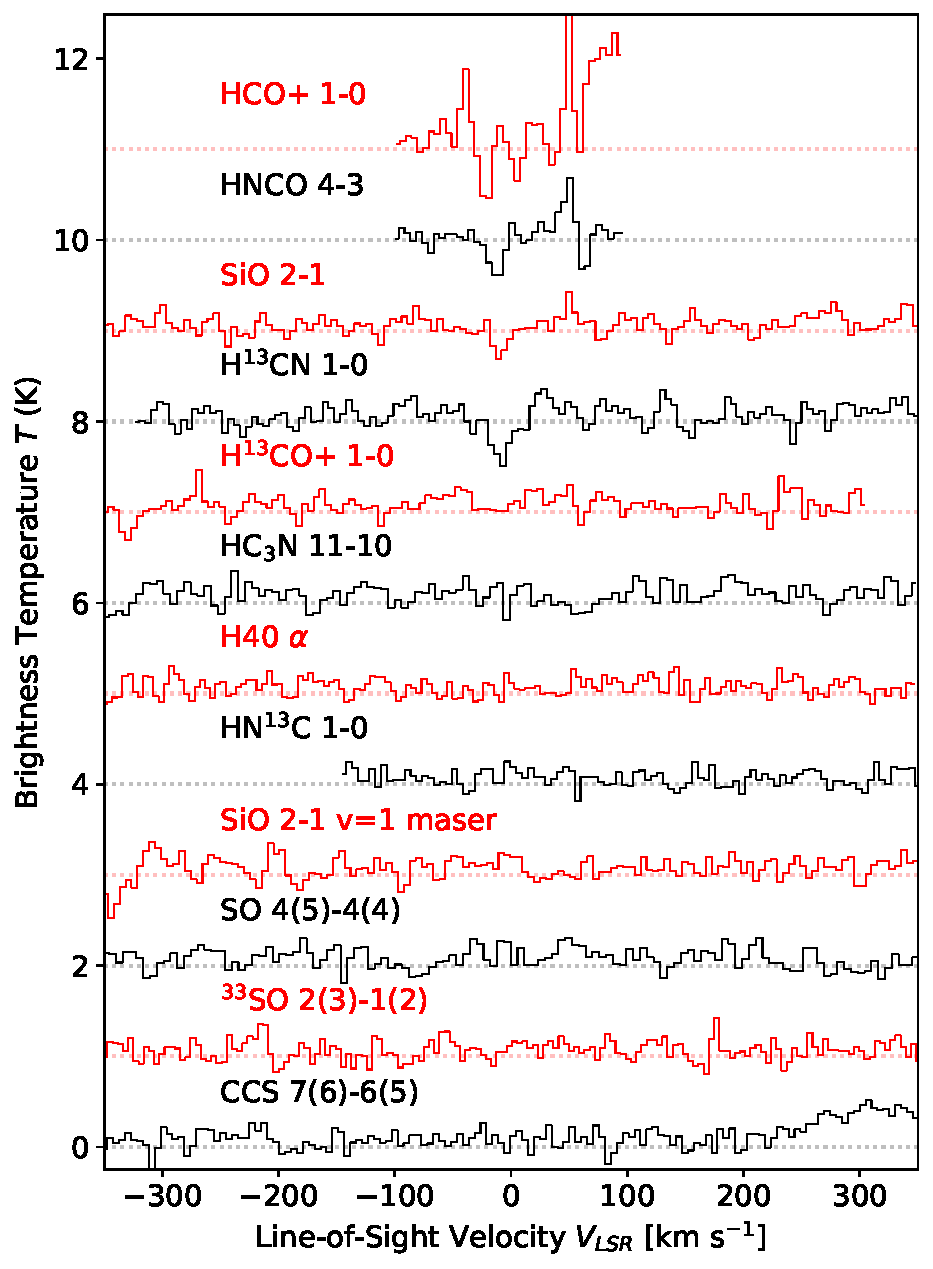
\includegraphics[width=0.49\textwidth]{figures/NonDetection_Overlays.pdf}
    \caption{Spectra of S-bearing lines in the ACES spectral coverage (left) and H-bearing or other lines (right).
    Only CS, SO, and SO$_2$ are detected.
    %Figure \ref{fig:coarse_spectra_withTP} shows the same data with the Total Power spectra, which covers larger physical scales ($\sim2$ pc), overlaid.
    }
    \label{fig:coarse_spectra}
\end{figure}


\begin{figure}
    \centering
    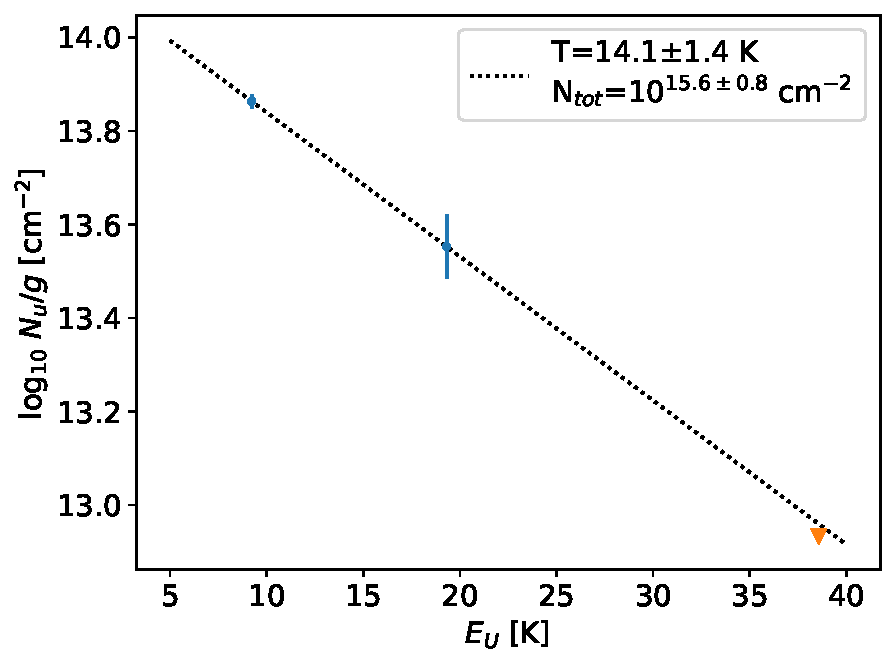
\includegraphics[width=0.49\textwidth]{figures/LTE_rotationdiagram_fit.pdf}
    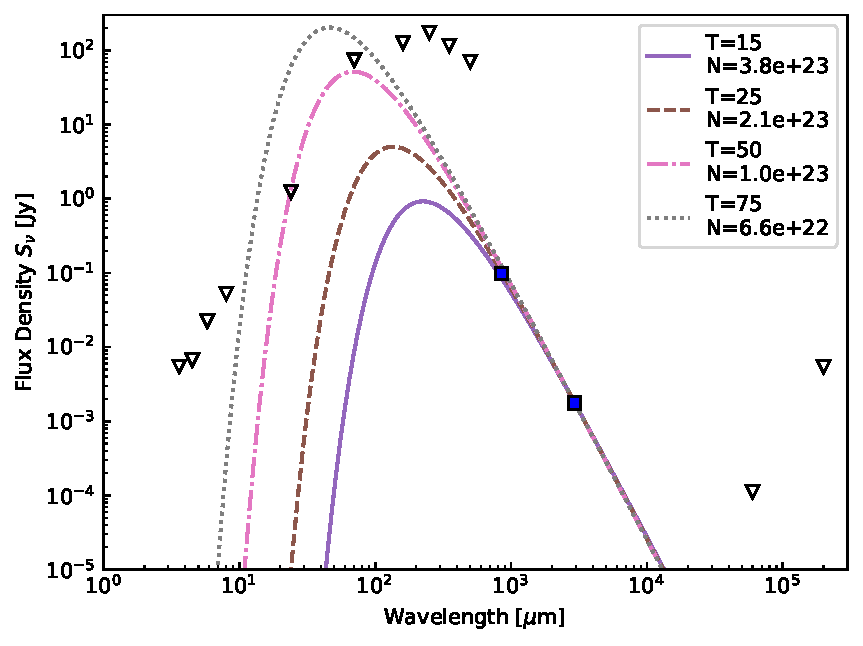
\includegraphics[width=0.49\textwidth]{figures/SED_with_upperlimits_VLA.pdf}
    \caption{(left) Rotation diagram showing the best fit for the SO lines.
    With only two lines, we cannot tell whether the lines are in LTE and genuinely cold or are instead sub-thermally excited.
    (right) Continuum spectral energy distribution. Except for the ALMA data points, all are upper limits.  The modified blackbody curves show that the dust temperature is limited to be $T_D<50$ K.
    }
    \label{fig:LTErotationdiagram}
\end{figure}


\begin{table}[htp]
    \centering
    \begin{tabular}{|c|c|c|c|c|c|c|c|}
         \hline
         Hypothesis & Broad & No IR & No X-ray & Gaussian & $X_{SO}$, $X_{CS}$ & No SiO & Size \\
         \hline
         IMBH \cellcolor{yellow!25} & \cellcolor{green!25}+ & \cellcolor{green!25}+ & \cellcolor{red!25}- & \cellcolor{red!25}- & & & \cellcolor{green!25}+\\
         \hline
         Stellar Merger \cellcolor{yellow!25} & \cellcolor{green!25}+ & \cellcolor{red!25}- & & & \cellcolor{green!25}+ & \cellcolor{red!25}-  & \cellcolor{green!25}+\\
         \hline
         YSO  \cellcolor{yellow!25} & \cellcolor{red!25}- &  \cellcolor{green!25}+ & & \cellcolor{green!25}+ & \cellcolor{red!25}- & \cellcolor{red!25}- &\cellcolor{green!25}+  \\
         \hline
         Protostellar Outflow \cellcolor{orange!25} & \cellcolor{green!25}+ & \cellcolor{red!25}- & & \cellcolor{red!25}- & \cellcolor{red!25}- & \cellcolor{red!25}-  & \cellcolor{red!25}-\\
         \hline
         Supernova \cellcolor{orange!25}& \cellcolor{green!25}+ & \cellcolor{green!25}+ & \cellcolor{red!25}- & & \cellcolor{red!25}- & \cellcolor{red!25}- & \\
         \hline
         (pre)Planetary Nebula \cellcolor{orange!25}& \cellcolor{red!25}- & \cellcolor{red!25}- & &  \cellcolor{green!25}+ & \cellcolor{green!25}+ & \cellcolor{red!25}- & \\
         \hline
         Background Galaxy \cellcolor{red!25}& \cellcolor{green!25}+ & \cellcolor{red!25}- & & & \cellcolor{red!25}- &  & \cellcolor{red!25}-\\
         \hline
         High-velocity Compact Cloud  \cellcolor{red!25}& \cellcolor{green!25}+ & \cellcolor{green!25}+ & \cellcolor{green!25}+ & \cellcolor{red!25}- & \cellcolor{red!25}- & \cellcolor{red!25}- & \cellcolor{red!25}-\\
         \hline
    \end{tabular}
    \caption{Hypotheses that have been evaluated and the evidence for (green +) and against (red -) them; blank means the evidence is neither for nor against.
    The overall weight given to the hypothesis is given by its color code - yellow are not entirely ruled out, orange are strongly disfavored but still possible, and red are very low likelihood.
    There is at least one strong item of evidence against each hypothesis considered.
    }
    \label{tab:hypotheses}
\end{table}



\section{Description of observations}

We will observe the target in B4 and B7 with 0.2" resolution to resolve the source, confirm its dusty nature, and measure the excitation in its lines.
While our observations will cover a wide range of species, we focus on the CS and SO molecules, since they are both clearly detected in existing B3 data.

% Please describe the observations to be made and their specific
% purpose, with a clear explanation of the need for, and 
% appropriateness of, ALMA Cycle 10 data.  

%No matter the nature of this source, it is clear that we need to follow it up.  The key observations to distinguish the above possibilities are:

% \begin{enumerate}
%     \item Resolved observations of the structure of the molecular feature.  We should aim for resolution $10\times$ better than currently achieved, which is straightforward with ALMA and can be requested at several wavelengths in the upcoming Configuration 6 in June 2024.  This is the key measurement, since the shape of the kinematic structure should be different for all of the above hypotheses (e.g., a circumstellar disk will have a Keplerian curve, while a galactic inner disk would likely be either solid-body or flat).  
%     \item A better molecular inventory.  Observations of HCN, HCO+, HNCO would be nice.  CO isotopologues, including very rare ones (C$^{17}$O, $^{13}$C$^{18}$O) should be included to avoid CMZ optical depth problems.  We should brainstorm other important species.  For example, H$_2$CS and H$_2$CO may be useful for better constraining the sulfur chemistry and the gas temperature.
%     \item A better physical characterization.  Additional transitions of CS and SO are necessary to measure the excitation.  Is the temperature really as low as we measure, or is the density low and we are instead seeing non-LTE conditions?
% \end{enumerate}

% TODO: mismatch in sensitivity...
Our sensitivity goal is to detect a 5 mJy signal in an 0.2" beam and a 5 \kms channel width at 5$\sigma$.
We adopt 5 \kms as our sensitivity target because, although the line is very broad, we need to detect it in many channels to measure the line shape, and we need to remove line-of-sight clouds from the profile before fitting.
This is a similar brightness sensitivity to the archival observations, but in a smaller beam so that we can confirm (or reject) the velocity gradient measurement.
The peak line intensity observed in B3 in the two brightest lines is 30 mJy in SO 3(2)-2(1) and 18 mJy in CS 2-1.

We target Band 3 and 7 to measure the dust spectral index and additional lines of both CS and SO at high resolution.
While we have a continuum detection in Band 7 with the ACA, it is at poor 4" resolution and does not resolve the continuum source or detect line emission.
The B7 data will achieve high signal-to-noise in the continuum with expected noise $\sigma_{350 GHz}=0.03$ mJy/beam yielding S/N $> 2000$ if the source remains unresolved.
The B4 data will have $\sigma_{140 GHz}\approx5$ $\mu$Jy, yielding predicted S/N$\sim1000$.
With this high signal-to-noise, we anticipate self-calibration will be needed to maximize the continuum sensitivity.


We performed basic RADEX modeling adopting the LTE-inferred column density N(SO) = $4\times10^{15}$ \persc and $T=13$ K.
The Band 4 SO 3(4)-2(3) line is the key diagnostics: 3(4)-2(3) will be detectable at $T_B>2.5$ K ($>5\sigma$) for T=13 K, $n\geq5\times10^4$ \percc, so we can use it to constrain the gas density.
There are several other SO lines in both bands that the RADEX model predicts will not be detected, but they come along for free.

The CS 3-2 and 7-6 provide an independent measurement of the rotational temperature and density conditions.
For T=13 K, CS 3-2 will be detected at $>5\sigma$ for $n\geq5\times10^5$ \percc; it should be detected for any plausible combination of physical parameters.
By contrast, the CS 7-6 line will only be detected if the density and temperature are both high ($n>10^6$ \percc, $T>50$ K), so it is an excellent diagnostic of high-excitation conditions.
%The model predicts the SO 8(8)-7(7) line will be 0.1 K (0.4 mJy) if SO is in LTE at 13 K, which is below our practical detection limit. 
% 
%and it would remain detectable down to $n(H_2)>5\times10^5$ \percc at the assumed temperature $T=13~K$.

\section{References}

% List references here
% Minimum font size for references: 12pt 
% Proposals not compliant to this will be rejected. See Section 5.3.1 in the ALMA Proposer's Guide.

\bibliography{main}{}
\bibliographystyle{aasjournal}


%%%%%%%%%%%%%%%%%%%%%%%%%%%
%%%%% End of document %%%%%
%%%%%%%%%%%%%%%%%%%%%%%%%%%

\end{document}

